\chapter{Metodología}
\label{cap:capitulo7}

\section{Requisitos}
\label{sec:requisitos}

Para dar respuestas a los objetivos planteados, este trabajo deberá cumplir los siguientes requisitos:

\begin{enumerate}
  \item Se utilizará \textit{GNU/Linux}, con la distribución \textit{Ubuntu 22.04 LTS}, como sistema operativo, en la plataforma hardware que se encargará de ejecutar el programa del sistema de visión.
  \item Los modelos entrenados se deben ajustar a las limitaciones del hardware que ejecutará el programa del sistema de visión.
  \item El sistema deberá poder ser utilizado en tiempo real. 
  \item El \textit{hardware} utilizado para el desarrollo del sistema de visión deberá ser lo suficientemente económico como para ser adquirido por cualquier estudiante.
  \item La aplicación debe ser fácilmente reproducible y desplegable tanto en un entorno simulado como en un ambiente educativo real o de laboratorio.
\end{enumerate} 

\section{Competencias}
\label{sec:competencias}

Las competencias adquiridas en el Grado de Ingeniería de Tecnologías Industriales que han sido utilizadas para la realización de este proyecto, se dividen tanto en generales como específicas, y son las siguientes:

\begin{enumerate} 
  \item \textit{Capacidad de organización y planificación: CG02.} Esta competencia ha sido empleada en la consecución de todo el trabajo de fin de grado, y queda reflejada tanto en las reuniones semanales o quincenales con el tutor responsable de este trabajo como en la wiki de GitHub\footnote{\url{https://github.com/RoboticsURJC/tfg-dcampoamor/wiki}} dedicada al proyecto, que refleja los avances y la organizacización llevada a cabo.  
  \item \textit{Conocimiento de una lengua extranjera: CG04.} Esta competencia ha sido utilizada a la hora de buscar toda clase de información para poder elaborar este proyecto, ya que se han utilizado documentos publicados en, al menos, una lengua extranjera, como lo es el inglés.
  \item \textit{Resolución de problemas: CG06.} Dado el nivel de conocimiento necesario en ciertas materias como la inteligencia artificial o la visión artificial, ha sido empleada para poder resolver los diversos inconvenientes que afrontar durante las pruebas prácticas relacionadas con estas áreas del trabajo.
  \item \textit{Uso de internet como medio de comunicación y como fuente de información: CG21.} Para poder elaborar este trabajo de fin de grado, ha sido necesario emplear esta competencia para buscar la información necesaria y poder completar principalmente los capítulos 1 y 2.
  \item \textit{Conocimientos de informática relativos al ámbito de estudio: CG24.} Esta competencia ha sido empleada a la hora de desarrollar y programar la aplicación sobre la que trata este trabajo.
  \item \textit{Conocimientos básicos sobre el uso y programación de los ordenadores, sistemas operativos, bases de datos y programas informáticos con aplicación en ingeniería: CE3.} Para poder desarrollar la aplicación se tuvo que emplear esta competencia a la hora de llevar a cabo la partición del disco duro en el ordenador y poder instalar la versión de \textit{Ubuntu 22.04.5 LTS (Jammy Jellyfish)}.  
  \item \textit{Conocimientos sobre los fundamentos de automatismos y métodos de control: CE13.} Esta competencia se refleja en la programación de la toma de decisiones automática, donde el sistema ajusta las operaciones en función de los resultados obtenidos del sistema de visión, así como el trabajo sincronizado de varios dispositivos (cámara y robot) y la comunicación entre estos.
  \item \textit{Conocimiento de los principios de regulación automática y su aplicación a la automatización industrial: CE32.} Esta competencia se emplea una vez que el sistema de visión identifica el grado de maduración de la fresa, ya que el sistema toma la decisión de recolectar o no el fruto, ajustando los actuadores o robots para realizar la tarea de forma precisa, dependiendo de las condiciones detectadas. Así mismo, se emplea la regulación automática en la optimización del proceso ajustando el comportamiento del robot en función del estado de la maduración de la fresa, maximizando la velocidad de la aplicación y su precisión.
  \item \textit{Capacidad para diseñar sistemas de control y automatización industrial: CE33.} Gracias a esta competencia se ha podido estructurar el sistema completo, incluyendo la parte de visión artificial, el procesamiento de imágenes, la toma de decisiones y el control del brazo robótico, integrando todos los datos en tiempo real y llevando a cabo operaciones de monitoreo y seguimiento de la aplicación y sus operaciones en remoto, tal y como se realizó en la etapa de pruebas.
  
\end{enumerate}  

Por otro lado, las competencias adquiridas con el desarrollo de este trabajo fin de grado, y que aparecen descritas en la guía docente de la propia asignatura, son las siguientes:

\begin{enumerate}
  \item \textit{Capacidad de análisis y síntesis: CG01.} Esta competencia se adquiere debido a la necesidad de la búsqueda y recopilación de información necesaria para el desarrollo del proyecto.
  \item \textit{Razonamiento crítico: CG11.} En relación con la competencia adquirida CG01, el razonamiento crítico se emplea a la hora de filtrar, seleccionar y decidir qué de toda la información obtenida es válido, cómo se puede utilizar y cómo ajustarlo y añadirlo al contenido del proyecto.
  \item \textit{Aprendizaje autónomo: CG13.} Esta competencia ha sido adquirida dada  la necesidad de adaptarse al marco técnico en cuál se desarrolla este proyecto, su complejidad, y la constante actualización y mejoras de las técnicas que pueden ser empleadas para el desarrollo del mismo.
  \item \textit{Adaptación a nuevas situaciones: CG14.} Esta competencia se adquiere gracias a la aplicación de la competencia adquirida \textit{CG13 Aprendizaje autónomo}, justificada anteriormente, y que se puede ver reflejada en el proyecto.
  \item \textit{Capacidad de aplicar los conocimientos teóricos en la práctica: CG20.} La parte empírica y práctica del proyecto refleja la adquisición de esta competencia.
  \item \textit{Capacidad para entender el lenguaje y propuestas de otros especialistas: CG22.} Esta competencia se ha visto reflejadas dado que, en relación con el resto de competencias adquiridas, sobre todo con las competencias \textit{CG01 Capacidad de análisis y síntesis} y \textit{CG11 Razonamiento crítico}, se ha tenido la necesidad de consulta, recopilación y filtrado de información y metodologías científicas existentes para poder desarrollar la aplicación del proyecto.
\end{enumerate} 


\section{Metodología}
\label{sec:metodologia}

Para lograr los objetivos descritos anteriormente, se optó por emplear el método DMADV (Definir, Medir, Analizar, Diseñar,Verificar), perteneciente a la metodología \textit{Six Sigma} (Figura \ref{fig:DMADV}). \\

Se decidió optar por esta metodología dado que la aplicación desarrollada en este trabajo está basada en otros proyectos y estudios similares ya existentes, y esta metodología está diseñada para desarrollar procesos o productos nuevos o significativamente mejorados, independientemente de si partes de cero o si te basas en conocimientos previos, y esta información recopilada fue utilizada como punto de partida en las fases iniciales de la metodología. A continuación, se detallan las fases del método DMADV y cómo han sido aplicadas en el desarrollo de este proyecto.

\begin{itemize}
  \item Definir: En esta fase se establecen como objetivos del proyecto la identificación de fresas maduras mediante un sistema de visión artificial y su integración con el brazo robótico encargado de su recolección. 
  \item Medir: Tomando como referencia el estado del arte existente, se llevó a cabo la selección de la tecnología (hardware y software necesarios) y las métricas existentes para poder considerar que las detecciones son aceptables y suficientes, basándose así el trabajo en proyectos y estudios que han demostrado ser eficaces, constituyendo un proyecto robusto y eficiente y ayudando a evitar problemas comunes ya que se sostiene sobre conocimientos adquiridos de proyectos similares testados. 
  \item Analizar: En esta etapa se llevaron a cabo pruebas con diferentes algoritmos y sistemas para detección de objetos, tanto en imágenes como en vídeo a tiempo real, para poder determinar cuál ofrecía un mejor rendimiento en precisión y velocidad y se ajustaba a los requisitos que presentaba el hardware disponible para el desarrollo del proyecto.  
  \item Diseñar: En base a los resultados obtenidos en la fase de análisis, se configuró el sistema de reconocimiento por visión incluyendo el hardware, previamente seleccionado, y el software, compuesto por los códigos y entornos necesarios para poder desarrollarlo y ejecutarlo, y su integración con el robot.
  \item Verificar: Finalmente, se llevaron a cabo pruebas para verificar que el sistema funcionaba y cumplía con los requisitos definidos, validándose la precisión en la identificación de las fresas maduras con distintas intensidades de luz ambiente y la comunicación y el correcto funcionamiento del brazo robótico.
\end{itemize}
  
\begin{figure} [H]
    \begin{center}
      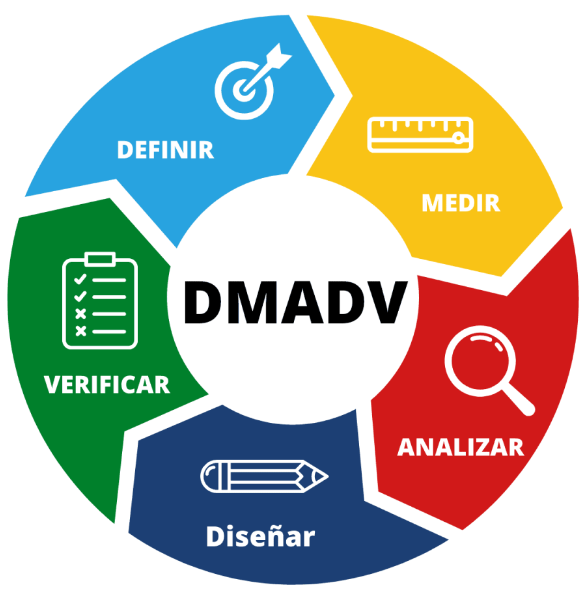
\includegraphics[width=7cm]{figs/DMADV.png}
    \end{center}
    \caption{Ciclo de la metodología DMADV}
    \label{fig:DMADV}
\end{figure}

\section{Habilidades desarrolladas}
\label{sec:habilidades_desarrolladas}

Además de todas las competencias descritas en la Sección \ref{sec:competencias}, a lo largo del desarrollo de este Trabajo Fin de Grado se han adquirido y reforzado numerosas habilidades y conocimientos, entre los cuales cabe destacar:

\begin{itemize}
    \item Se ha adquirido una sólida capacidad de organización y planificación, debida a la estructuración del proyecto, el seguimiento mediante reuniones periódicas con el tutor y la documentación detallada de los avances en la plataforma GitHub.
    \item Se ha mejorado notablemente la capacidad de búsqueda, análisis y síntesis de información técnica en inglés, utilizando documentación científica y recursos especializados en visión artificial, inteligencia artificial y robótica.
    \item Se ha fortalecido la competencia en resolución de problemas, especialmente al afrontar desafíos técnicos relacionados con el entrenamiento de modelos de Machine Learning, la calibración del sistema de visión o la integración del sistema con el robot.
    \item Se ha desarrollado la habilidad de utilizar Internet como fuente de información académica y técnica, contrastando distintas metodologías y enfoques para fundamentar las decisiones adoptadas en el diseño del sistema.
    \item Se han adquirido conocimientos avanzados en programación en Python, además de conocimientos básicos en el uso de bibliotecas específicas como OpenCV, OpenGL, PyTorch y en herramientas de comunicación como XML-RPC.
    \item Se ha reforzado el uso y conocimiento sobre el sistema operativo GNU/Linux, ya que, partiendo desde la instalación y configuración de Ubuntu 22.04 LTS y la gestión de particiones del disco duro del ordenador utilizado en la elaboración del proyecto, se ha hecho uso de la terminal y de conexiones remotas vía SSH a partir de esta.
    \item Se han desarrollado competencias en la recogida, tratamiento y etiquetado de datos para el entrenamiento de modelos de inteligencia artificial, construyendo un dataset propio de imágenes de fresas.
    \item Se ha adquirido la habilidad de entrenar y optimizar modelos de aprendizaje supervisado adaptados a plataformas con recursos limitados, asegurando su funcionamiento en tiempo real.
    \item Se ha aprendido a integrar un sistema de visión con un brazo robótico, automatizando la toma de decisiones a partir de los datos recogidos por la cámara.
    \item Se ha reforzado el conocimiento de los fundamentos de la automatización industrial y la regulación automática, aplicados a la ejecución precisa de tareas por parte del robot en función del estado de maduración detectado en cada fresa.
    %\item Se ha desarrollado la capacidad para diseñar e implementar sistemas de control en tiempo real, integrando múltiples componentes en una solución funcional y coordinada.
    \item Finalmente, se ha adquirido experiencia en la redacción técnica y científica, mediante el uso de LaTeX para la elaboración de la memoria del proyecto, cuidando la estructura, el lenguaje y el formato exigido en un entorno académico.
\end{itemize}
